\documentclass[10.5pt]{article}
\usepackage[margin=0.76in]{geometry}
\usepackage{amsmath,amssymb,booktabs,tabularx,array,graphicx,caption,microtype,xcolor,xurl,hyperref,longtable,enumitem}
\usepackage[T1]{fontenc}
\definecolor{linkblue}{HTML}{356AA0}
\definecolor{warnorange}{HTML}{D9822B}
\definecolor{goodgreen}{HTML}{3B7D67}
\hypersetup{colorlinks=true,linkcolor=linkblue,urlcolor=linkblue,citecolor=linkblue}
\newcommand{\R}{\mathbb{R}}
\newcommand{\E}{\mathbb{E}}
\newcommand{\orth}{\mathrm{ORTH}}
\newcommand{\plug}{\mathrm{PLUG}}
\newcommand{\riesz}{\mathrm{RIESZ}}
\newcommand{\pass}{\textcolor{goodgreen}{\textbf{pass}}}
\newcommand{\conditional}{\textcolor{linkblue}{\textbf{conditional}}}
\newcommand{\fail}{\textcolor{warnorange}{\textbf{fail}}}
\newcolumntype{Y}{>{\raggedright\arraybackslash}X}
\setlist{nosep,leftmargin=1.4em}
\graphicspath{{figures/}{../distributional_sid_decisive_2026-07-14/figures/}}

\title{\textbf{Adjudicating the Distributional SID Experiments}\\
\large Failure analysis, missing baselines, parameter/data scaling, and revised conclusions}
\author{Synthetic-methods audit and post-hoc validation}
\date{July 14, 2026}

\begin{document}
\maketitle

\begin{abstract}
The first decisive validation of predictive distributional Jacobians found regular-case successes but apparent failures under heavy tails/weak overlap (E6), filtering (E8), and dense response geometry (E9).  This report asks whether those failures reflect the estimand and orthogonal-score theory, the synthetic design, or the particular nuisance/readout implementation.  We added development-only parameter searches and unused-seed post-hoc sample/horizon/dimension scaling, exact characteristic deconvolution, a correctly specified measurement-model likelihood, a direct learned density-score representer, an effective-rank audit, oracle inversion sweeps, and a 30-seed high-dimensional replication.  The audit adds 7,615 rows with zero failed fits or duplicate rows; all run validators and 20 package tests pass.

The revised answer is more favorable but narrower.  The fixed targeted Riesz sieve fails, not the E6 estimand: a learned density-score representer plus ORTH removes the bias in the tested low-dimensional tail/gap families as data grow.  Severe filtering is recoverable only with a long enough observation window and a correct measurement model; the four-step case remains information-limited.  E9's nominal rank-three generator was population rank two, and its characteristic inversion ridge was four orders of magnitude too large.  After correcting both issues, direct/low-rank covariance heads recover the intended geometry; characteristic inversion recovers the same typed covariance after retuning but gives no point-error benefit, while its full feature tangent remains noisy.  The overall recommendation is therefore to develop a modular SID framework: ORTH bounded features for broad declared queries, density-score/Riesz diagnostics for history integration, measurement-aware inversion only when conditioning permits it, and structured typed heads for known geometry.  It is not evidence for unrestricted full-law or latent neural recovery.
\end{abstract}

\section{Executive answer}

\paragraph{What works best.}
For a known low-dimensional target, the best default remains a calibrated direct head.  For many bounded characteristic/path features under regular support, the cross-fitted ORTH estimator is the best-developed reusable observational method because it supplies valid uncertainty and works through support motion.  For E6-style observational derivatives, the promising nuisance learner is now \emph{direct density-score estimation}, not the original targeted random-feature Riesz sieve.  For dense covariance geometry, a direct low-rank covariance head is decisively preferable to first estimating a large characteristic tangent and then inverting it.  For filtered latent dynamics, exact characteristic deconvolution is useful only after the observation horizon makes the inverse problem well conditioned and the measurement model is credible.

\paragraph{What the apparent failures meant.}
They were not one thing:
\begin{itemize}
\item E6 was mainly \textbf{fixed-sieve misspecification}; more data alone made its undercoverage more obvious.  Changing the representer learner produced sample-scaling improvement.
\item E8 mixed an \textbf{incorrect ``deconvolution'' implementation} (point projection), a weak filter estimator, and a genuine short-horizon information limit.  Exact characteristic correction plus a strong fitted measurement model works at long horizon, not at short horizon.
\item E9 combined an \textbf{unidentified synthetic rank}, an \textbf{over-regularized inverse readout}, and a genuinely high-variance full feature tensor.  The first two were design/implementation problems; the last is a real statistical limitation.
\end{itemize}

\paragraph{How much confidence to attach.}
The original frozen confirmations remain the confirmatory evidence.  The additional studies in this report are explicitly post-hoc adjudications using unused seeds.  They demonstrate which failures have hope and identify concrete repairs; they do not retroactively convert a failed preregistered gate into a confirmatory pass.  The new conclusions should be confirmed once more on frozen, non-home-field high-dimensional generators.

\begin{table}[t]
\centering
\scriptsize
\renewcommand{\arraystretch}{1.13}
\caption{Revised gate matrix after failure adjudication.  ``Conditional'' always refers to the tested access/model/horizon regime.}
\begin{tabularx}{\textwidth}{@{}p{0.46cm}p{2.6cm}p{2.65cm}Y@{}}
\toprule
ID & Question & Revised decision & Evidence and consequence \\
\midrule
E0 & Algebra/software/leakage & \pass & 20/20 package tests and every new run validator pass. \\
E1 & Regular equal-access recovery & \pass, no point win & ORTH NRMSE 0.104 and coverage 0.940; error ratio versus PLUG 1.002. \\
E2 & Orthogonal remainder & \pass & Product-order bias relation has $R^2>0.99999997$. \\
E3 & One future/dependence & \pass{} with HAC & At $\rho=.9$, NRMSE is 0.145/0.093 and HAC coverage 0.949/0.951. \\
E4 & Moment-blind law change & \pass{} at resolving bank & Power 1.00/0.867; moment FWER 0.067/0.067. \\
E5 & Support motion & \pass & ORTH NRMSE 0.016 at zero noise where the likelihood score is undefined. \\
E6 & Tails/weak overlap & \conditional{} rescue & Original sieve stays biased; density-score ORTH reaches error 0.0036 and coverage 1.00 in gap-4 at $n=128$k. \\
E7 & Heterogeneous cancellation & \pass{} at $R=2$ & Energy 3.982 versus 4.000 and sign reversal recovered. \\
E8 & Filtered latent recovery & \conditional{} rescue & At $\rho=.98,T=64,n=32$k, fitted-model CF ORTH NRMSE is 0.141; at $T=4$ it is 2.88. \\
E9 & Dense geometry & typed \pass; full-feature \fail & Identified $d_Y=8$ direct NRMSE 0.106 at 128k; $d_Y=32$ low-rank NRMSE 0.177 at 32k; full feature NRMSE remains about 1.01. \\
E10 & Flexible-law baselines & \pass{} pooled/local & Five MDN/NSF baselines, seven families, ten seeds, three initializations; no universal cell winner. \\
E11 & Path ordering & \pass & Full-path power 1.00; endpoint/unordered FWER 0.056. \\
\bottomrule
\end{tabularx}
\end{table}

\clearpage
\section{What the methods estimate}

Let $H\in\R^{d_H}$ be an observed history, $Y^{[T]}$ a future path, and $\Phi(Y^{[T]})\in\R^q$ a declared bounded feature map.  The common feature target is
\begin{align}
m(h) &= \E\{\Phi(Y^{[T]})\mid H=h\},\\
A_p &= \E\{\partial_{h_p}m(H)\}.
\end{align}
With a history basis $b_r(H)$, the heterogeneous target is $A_{r,p}=\E\{b_r(H)\partial_{h_p}m(H)\}$.  A Riesz representer $\alpha_{r,p}$ satisfies
\begin{equation}
\E\{\alpha_{r,p}(H)g(H)\}=\E\{b_r(H)\partial_{h_p}g(H)\}.
\end{equation}
The three matched estimators are
\begin{align}
\plug &: \quad \partial_{h_p}\widehat m(H),\\
\riesz &: \quad \widehat\alpha_{r,p}(H)\Phi(Y),\\
\orth &: \quad b_r(H)\partial_{h_p}\widehat m(H)+\widehat\alpha_{r,p}(H)\{\Phi(Y)-\widehat m(H)\}.
\end{align}
All are cross-fitted in the main experiments.  ORTH is not supposed to beat PLUG in every regular point-estimation cell.  Its advantage is first-order insensitivity to nuisance errors:
\begin{equation}
\operatorname{Bias}(\widehat A_{\orth})\approx-\E\{(\widehat\alpha-\alpha)(\widehat m-m)\}.
\end{equation}
That protection disappears if one nuisance converges to a fixed wrong function.  This single fact explains much of E6.

\begin{table}[t]
\centering
\footnotesize
\renewcommand{\arraystretch}{1.12}
\caption{Method families, quantities, and fair roles.}
\begin{tabularx}{\textwidth}{@{}p{2.7cm}p{3.15cm}p{2.4cm}Y@{}}
\toprule
Method & Quantity learned & Objective & Proper role \\
\midrule
PLUG feature head & $m(h)=\E(\Phi\mid h)$ & bounded-feature regression & Same-target baseline; naive plug-in SE is generally incomplete. \\
Targeted Riesz & $\alpha(H)$ for derivative functional & empirical Riesz loss & History-side integration; original fixed sieve is E6's weak point. \\
Density-score Riesz & $\alpha=-\nabla\log p_H$ for $b=1$ & GMM density likelihood/score & Alternative E6 representer learner; low-dimensional post-hoc evidence. \\
ORTH & $A$ through $m$ and $\alpha$ & cross-fitted orthogonal score & Primary reusable bounded-feature estimator and inference route. \\
Direct typed head & mean/covariance/moment target & target-specific regression & Best baseline when the downstream target is known. \\
MDN & normalized conditional density & maximum likelihood & Reusable-law baseline with exact/autodiff characteristic readout. \\
NSF flow & normalized conditional density & maximum likelihood & Flexible reusable-law baseline; derivative estimated through samples. \\
Diffusion/DSM & noisy response score/generator & denoising score matching & Earlier score-tangent family; generative quality does not guarantee mixed history derivatives. \\
Flow matching & conditional transport field & flow-matching loss & Earlier generative family; same warning about tangent readout. \\
Ratio/classifier & finite density ratio/witness & classification & Appropriate for finite contrasts; not identical to an infinitesimal observational derivative. \\
\bottomrule
\end{tabularx}
\end{table}

\subsection{Access-tier discipline}
Oracle $m$, oracle $\alpha$, oracle Riesz, latent-state access, known filters, and oracle response subspaces are diagnostic ceilings, never learned competitors.  Learned comparisons share histories, futures, feature/query banks, evaluation histories, and random seeds within each cell.  Direct heads receive the target definition but no extra latent information.  E10 MDNs and spline flows are observational normalized-law baselines at the same local training sample and feature readout.

\section{Validation and audit trail}

The new program separated tuning from adjudication.  E6 width/ridge selection and E9 oracle inverse tuning used development-only cells/seeds.  The sample/horizon/dimension studies used unused post-hoc seeds 2001--2010; the $d_Y=32$ direct-geometry cell was replicated on 2011--2030, yielding 30 independent seeds.  These are diagnostic expansions motivated by the first confirmation and are labeled accordingly.

Across the ten adjudication run directories there are 7,615 seed-level rows.  Every run-level expected/observed-row check passes, every fit status is ``ok,'' all required reported metrics are finite, no seed-level file contains a duplicate full row, and SHA-256 hashes are recorded in \texttt{tables/validation\_audit.csv}.  The complete Python test suite passes 20/20.  The machine guard ran the heavier jobs sequentially, checked free disk and resident memory, and avoided another large neural run after baseline coverage was already complete.

\section{The original result landscape}

The first report remains the definitive description of E0--E11.  Its essential results are shown here so the adjudication is interpretable without switching documents.

\begin{figure}[t]
\centering
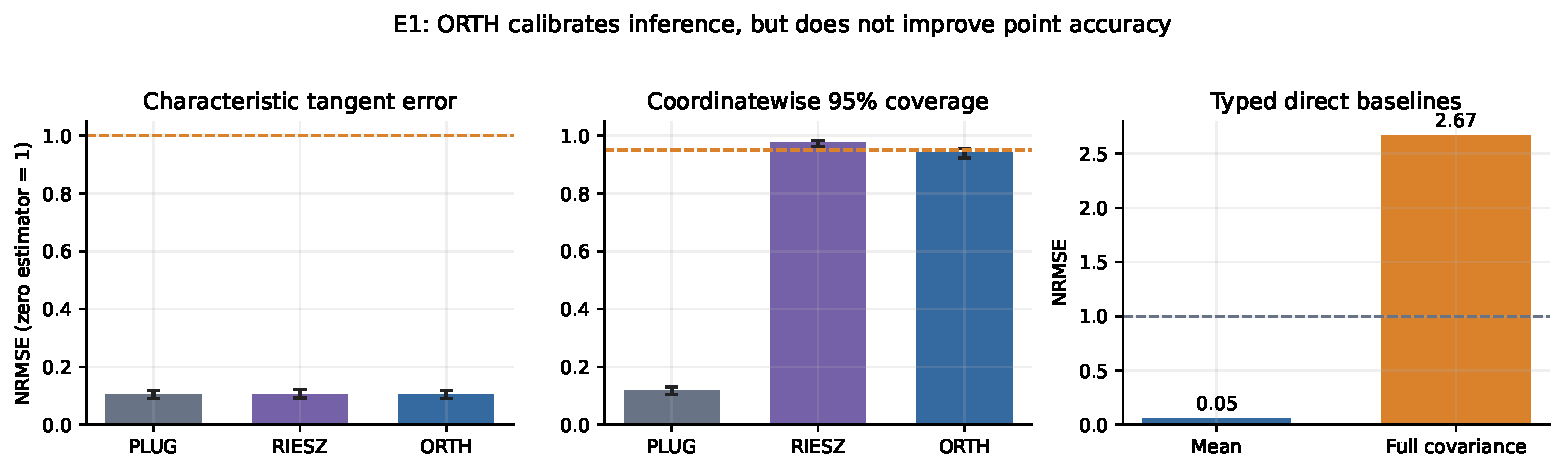
\includegraphics[width=\textwidth]{e1_recovery.pdf}
\caption{E1.  ORTH improves inference rather than point accuracy on the regular Gaussian reference; a direct mean head is strongest when the target is known.}
\end{figure}

\begin{figure}[t]
\centering
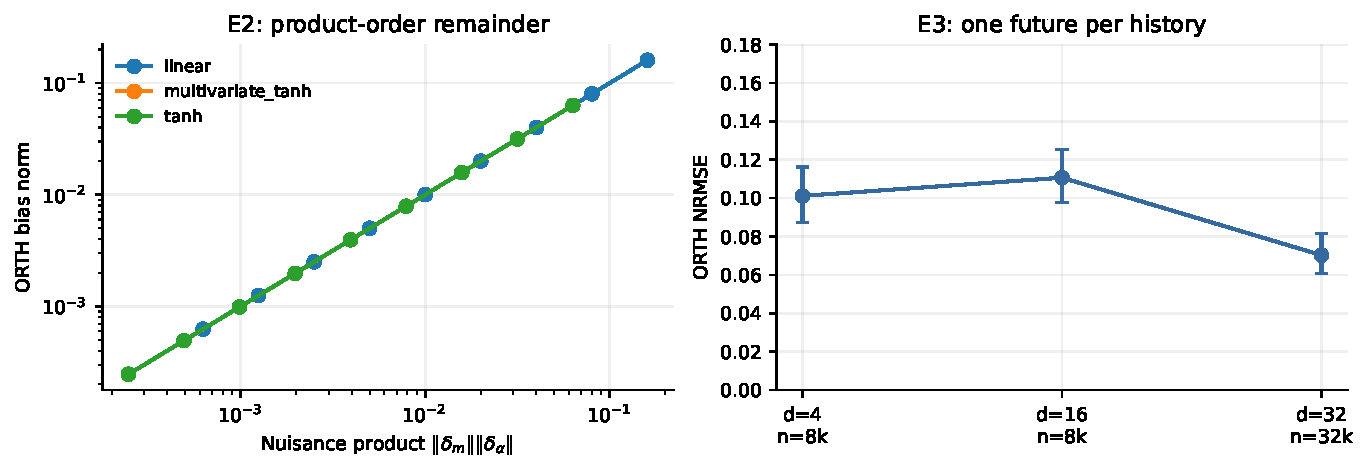
\includegraphics[width=0.92\textwidth]{e2_e3_orthogonality_scaling.pdf}
\caption{E2--E3.  Controlled product-order nuisance bias and stable one-future-per-history estimation; temporal dependence requires blocked splitting and HAC uncertainty.}
\end{figure}

E4 supplies a genuine but resolution-dependent advantage over a fixed first-four-moment list.  E5 is the clearest theoretical win: bounded weak features remain regular when a likelihood response score diverges or ceases to exist.  E7 shows that a global zero derivative can hide local sign reversals.  E11 shows that path features detect ordering that endpoints and unordered totals cannot.

\begin{figure}[t]
\centering
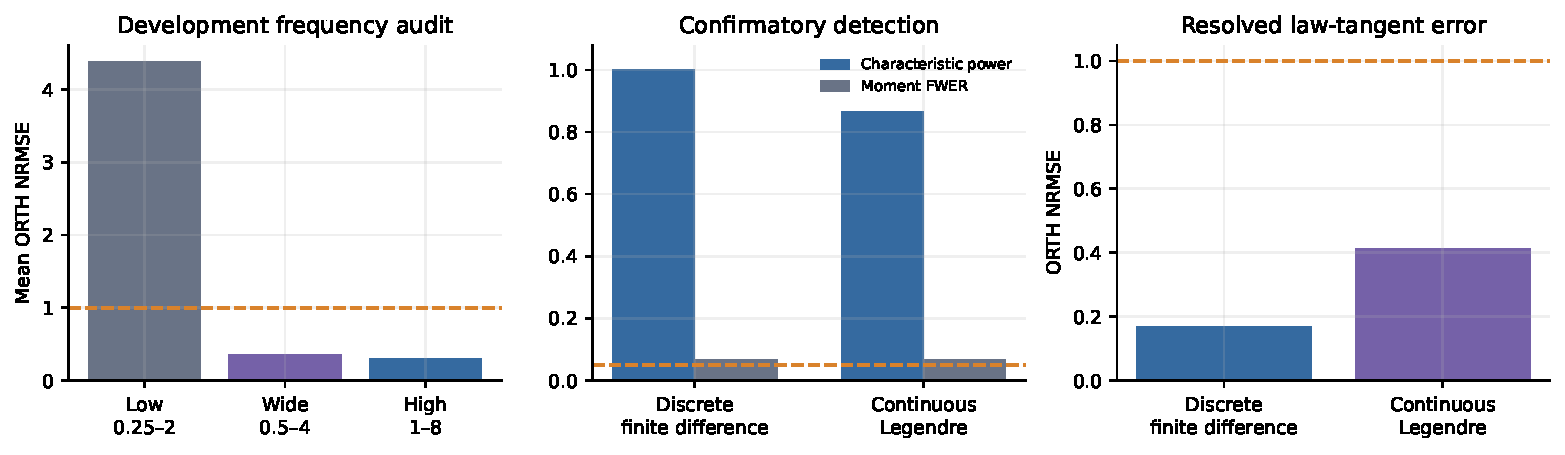
\includegraphics[width=\textwidth]{e4_frequency_moment_blind.pdf}
\caption{E4.  The default low-frequency bank missed a designed high-order departure; a frozen resolving bank detected it on new seeds.}
\end{figure}

\begin{figure}[t]
\centering
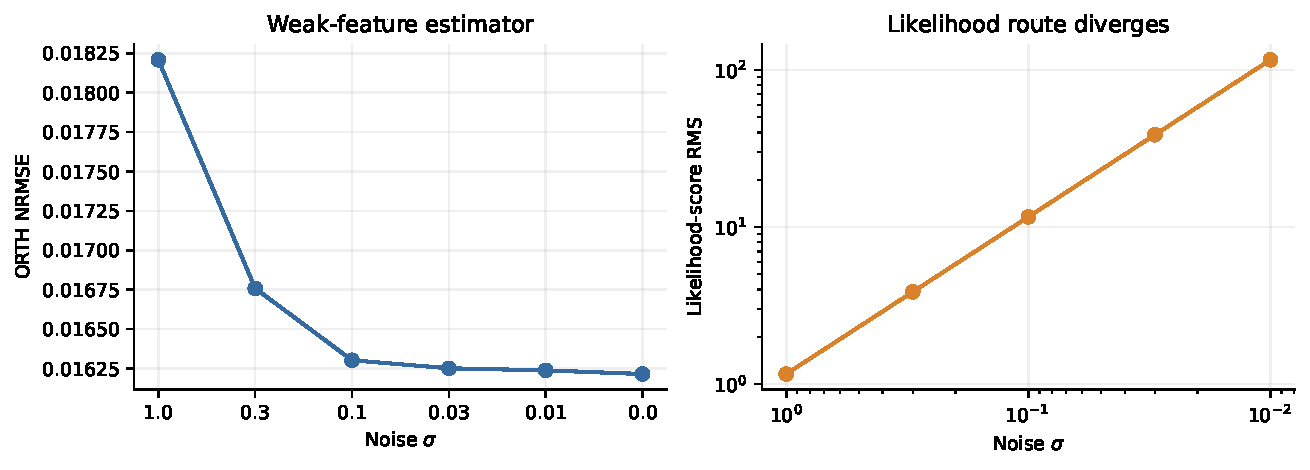
\includegraphics[width=0.90\textwidth]{e5_support_motion.pdf}
\caption{E5.  Weak-feature derivatives remain stable through deterministic support motion; the likelihood-score route scales like $1/\sigma$ and becomes undefined.}
\end{figure}

\begin{figure}[t]
\centering
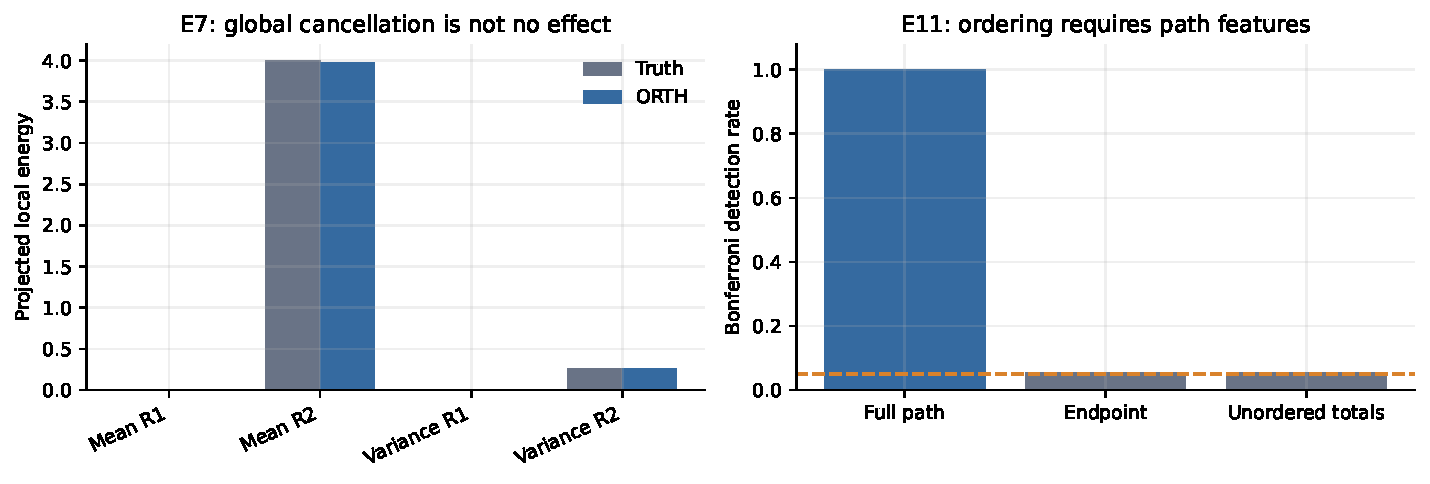
\includegraphics[width=0.94\textwidth]{e7_e11_heterogeneity_path.pdf}
\caption{E7 and E11.  History resolution reveals cancellation; future-path features recover ordering invisible to endpoint/unordered summaries.}
\end{figure}

\clearpage
\section{E6 adjudication: the representer learner failed}

\subsection{Why the original sieve could not be rescued by $n$ alone}

For $b(H)=1$ and a smooth history density, integration by parts gives
\begin{equation}
\alpha(H)=-\nabla_H\log p_H(H).
\end{equation}
The original implementation instead minimized a regularized Riesz loss in a fixed random-feature sieve.  In tail and low-density-bridge regions the true representer is large and structured, while the fixed ridge/sieve shrinks it toward a low-norm approximation.  ORTH only removes first-order nuisance error around the true nuisance.  If $\widehat\alpha\to\alpha_\star\ne\alpha$, its bias need not vanish.  More data then shrinks the standard error around a biased limit, so coverage can deteriorate.  That is exactly what the targeted gap-4 sequence shows: representer NRMSE stays near 0.966, absolute target error grows from 0.0220 to 0.0272, and coverage falls from 0.70 to zero between 8k and 128k.

\subsection{What was changed}

A development grid varied sieve width $32/64/128$ and Riesz ridge $10^{-3}/10^{-2}/10^{-1}$ using held-out probe residual, not oracle target error.  Width 128 and ridge $10^{-3}$ were frozen for the post-hoc sample ladder.  More importantly, a direct history-density route fitted a BIC-selected Gaussian mixture and differentiated its log density, producing a learned density-score representer.  Every method then used the same cross-fitted ORTH score and the same data.  Oracle Riesz was retained to separate approximation bias from irreducible overlap variance.

\begin{figure}[t]
\centering
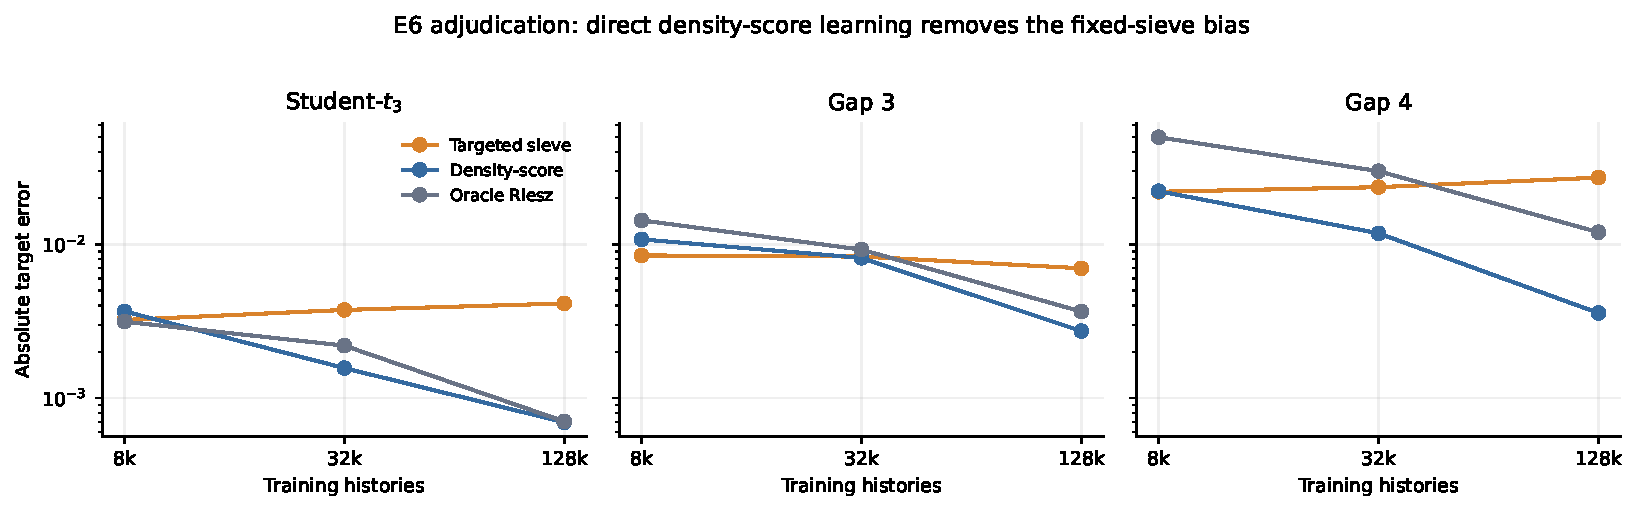
\includegraphics[width=\textwidth]{e6_sample_scaling.pdf}
\caption{E6 sample scaling.  In Student-$t_3$ and gaps 3--4, the density-score learner improves with data while the targeted fixed sieve reaches a bias floor.  The oracle curve shows that severe overlap also increases variance.}
\end{figure}

\begin{figure}[t]
\centering
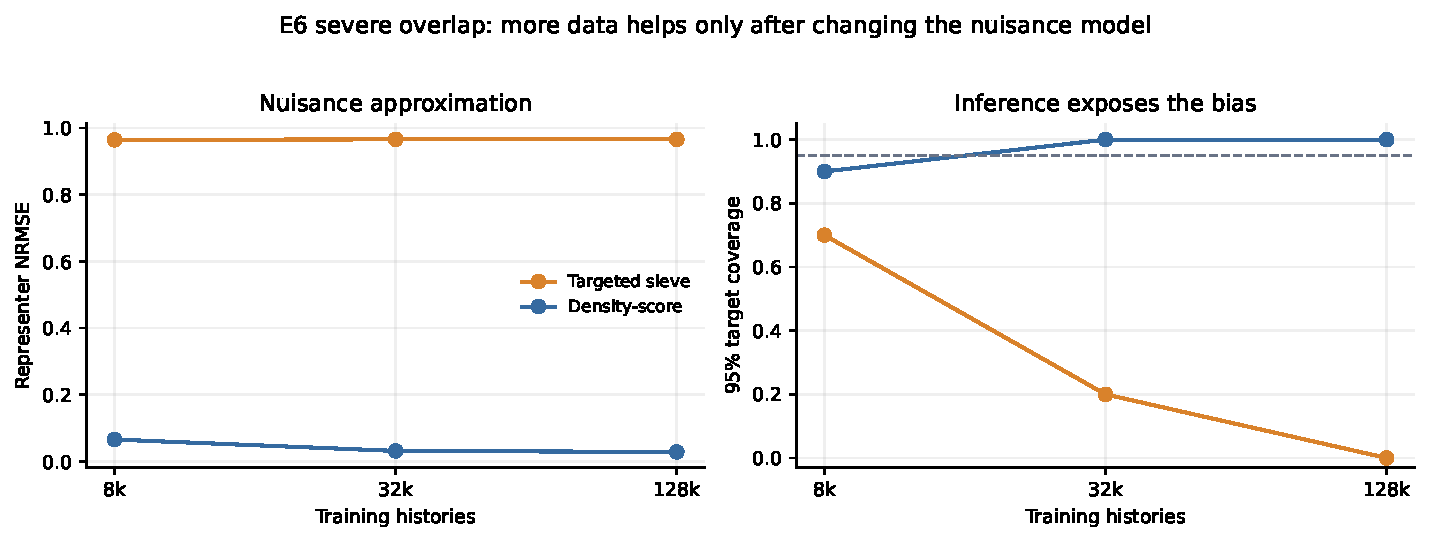
\includegraphics[width=0.90\textwidth]{e6_gap4_diagnosis.pdf}
\caption{Gap-4 diagnosis.  The alternative representer learner lowers nuisance NRMSE from about 0.966 to 0.029 and restores empirical target coverage; the original sieve's shrinking standard errors expose its fixed bias.}
\end{figure}

\subsection{Results and conclusion}

At $n=128$k, density-score ORTH has absolute target error 0.00070 for $t_3$, 0.00090 for $t_5$, 0.00273 for gap 3, and 0.00357 for gap 4, with empirical coverage 1.00, 0.90, 1.00, and 1.00 across ten seeds.  The targeted sieve has errors 0.00412, 0.00138, 0.00698, and 0.02719, with coverage 0.10, 0.80, 0.40, and zero.  In gap 4 the oracle representer norm is about 6.49 and oracle-Riesz error remains 0.012 at 128k, confirming that overlap makes the problem intrinsically noisy even when the nuisance is known.

This gives the approach real hope, but it is not yet a general pass.  The rescue uses low-dimensional history distributions that a Gaussian mixture can approximate.  The next confirmation must learn the history score in nonlinear, correlated, higher-dimensional trajectory distributions without using the DGP family and must retain explicit support/overlap refusal rules.

\section{E8 adjudication: a measurement inverse problem}

\subsection{What was wrong with the first correction}

The earlier ``known deconvolution'' projected the filtered observations back to a point estimate and applied the feature map.  That is not exact characteristic deconvolution.  If the observation window obeys a linear-Gaussian model
\begin{equation}
X_{1:T}=k_T Z+\epsilon,\qquad \epsilon\sim N(0,\sigma^2I),
\end{equation}
then
\begin{equation}
\varphi_X(u\mid h)=\varphi_Z(k_T^\top u\mid h)\exp\{-\tfrac12\sigma^2\|u\|^2\}.
\end{equation}
Exact recovery divides by the Gaussian attenuation at matched query directions.  Its variance is amplified by the reciprocal attenuation; this can be enormous when a short, strongly filtered window carries little information about $Z$.  A correct formula therefore does not remove an information limit.

\subsection{What was added}

The new grid crosses $\rho\in\{.9,.98\}$, horizons $T\in\{4,16,64\}$, $n\in\{8$k,$32$k$\}$, low/wide query banks, and ten post-hoc seeds.  It includes latent oracle features; point projection; exact CF deconvolution; known, moment-estimated, and correctly specified mixture-likelihood filter estimates; PLUG/RIESZ/ORTH decompositions; and zero controls.  The mixture likelihood integrates over the latent Bernoulli state and uses the correct observation noise family.  It estimates $\rho$ rather than receiving it.

\begin{figure}[t]
\centering
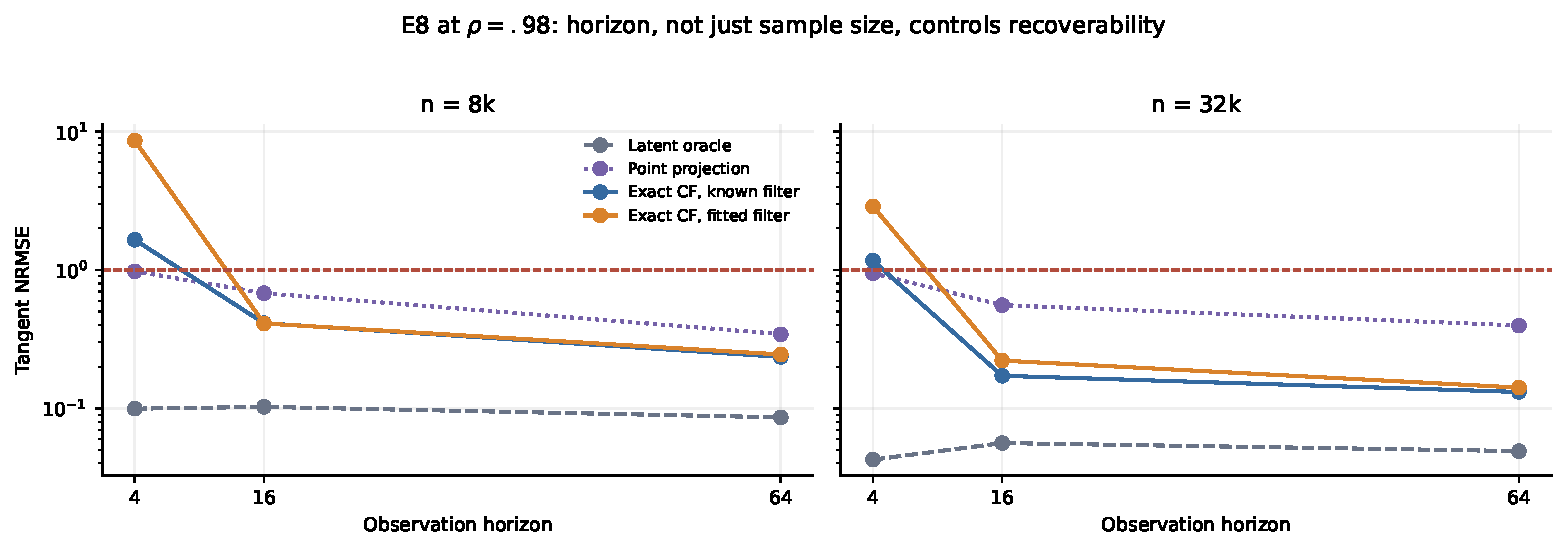
\includegraphics[width=\textwidth]{e8_horizon_deconvolution.pdf}
\caption{E8 at $\rho=.98$.  Longer observation windows change the conditioning enough to make exact characteristic recovery useful.  Sample size helps only after the horizon crosses that information threshold.}
\end{figure}

\begin{figure}[t]
\centering
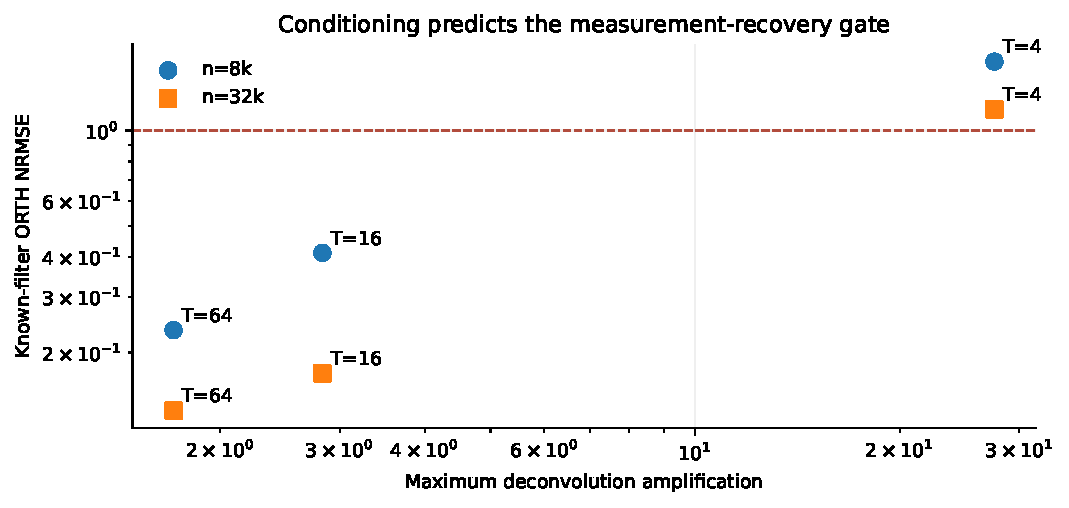
\includegraphics[width=0.76\textwidth]{e8_conditioning.pdf}
\caption{Known-filter cells: maximum inverse attenuation tracks the error regime.  This diagnostic should be reported before interpreting a corrected latent effect.}
\end{figure}

\subsection{Results and conclusion}

At $\rho=.98$ with the wide bank and known filter, exact CF ORTH NRMSE changes from 1.652 to 0.412 to 0.235 at $n=8$k as the horizon grows from 4 to 16 to 64.  At $n=32$k the sequence is 1.169, 0.172, and 0.131.  The latent oracle at $T=64,n=32$k is 0.049; a gap remains, but the latent target is clearly recoverable.  Point projection at the same cell is 0.396, three times worse than exact characteristic correction.

The mixture-likelihood estimator recovers $\rho$ very accurately: at $T=64,n=32$k its mean absolute error is $5.5\times10^{-4}$.  Its exact CF ORTH NRMSE is 0.141 with coverage 0.992.  At $T=4,n=32$k, despite $\rho$ error 0.0018, NRMSE is 2.88 because inverse attenuation averages about 67 at the maximum query.  Thus filter-parameter accuracy is not the same as target identifiability.

E8 is now a conditional success: matched measurement modeling and adequate horizon can recover the latent characteristic target.  It remains a hard deployment gate because the earlier misspecified-filter experiment collapsed coverage to 0.003, and the new rescue uses the correct observation family.  Future work should stress non-Gaussian, nonlinear, heteroskedastic, state-dependent, and misspecified sensors and report partial-identification or refusal when the inverse attenuation is too large.

\clearpage
\section{E9 adjudication: synthetic rank, inversion ridge, and target choice}

\subsection{The nominal rank-three generator was rank two}

In the gain-mixture construction, a Bernoulli component with probability $p(h)=\operatorname{logit}^{-1}(w^\top h+c)$ contributes a covariance coefficient proportional to $p(1-p)$.  Its history derivative contains
\begin{equation}
p(1-p)(1-2p)w.
\end{equation}
At $c=0$ with a symmetric Gaussian history distribution, this is an odd function of $w^\top H$, so its population average is zero.  The original symmetric intercept design therefore had effective response rank two even though three gain directions were simulated.  Its minimum population coefficient singular value is about $2\times10^{-6}$ and its response condition number is about $8\times10^{10}$.  Penalizing an estimator for not recovering three directions was invalid.

An identified intercept scheme $(-1.2,-0.4,0.9)$ has effective rank three, minimum singular value about 0.016, and condition number about 15.5.  All revised point-geometry claims use the effective population rank and report nominal/effective discrepancies.

\subsection{The characteristic inverse was over-regularized}

The typed covariance readout solves a linear inverse problem from characteristic derivatives.  The original ridge was $10^{-4}$.  In an oracle sweep over query counts 64/256, three frequency bands, and ridges $10^{-8}/10^{-6}/10^{-4}$, the best covariance NRMSE is 0.00471 at 256 low-frequency queries and ridge $10^{-8}$.  With the old 64-current/$10^{-4}$ setting, oracle NRMSE is 0.667 and the response angle is 47 degrees.  With the same 64-current bank but ridge $10^{-8}$, oracle NRMSE is 0.0111 and angle 0.28 degrees.  This is an implementation-scale failure, not a limitation of the population characteristic identity.

\begin{figure}[t]
\centering
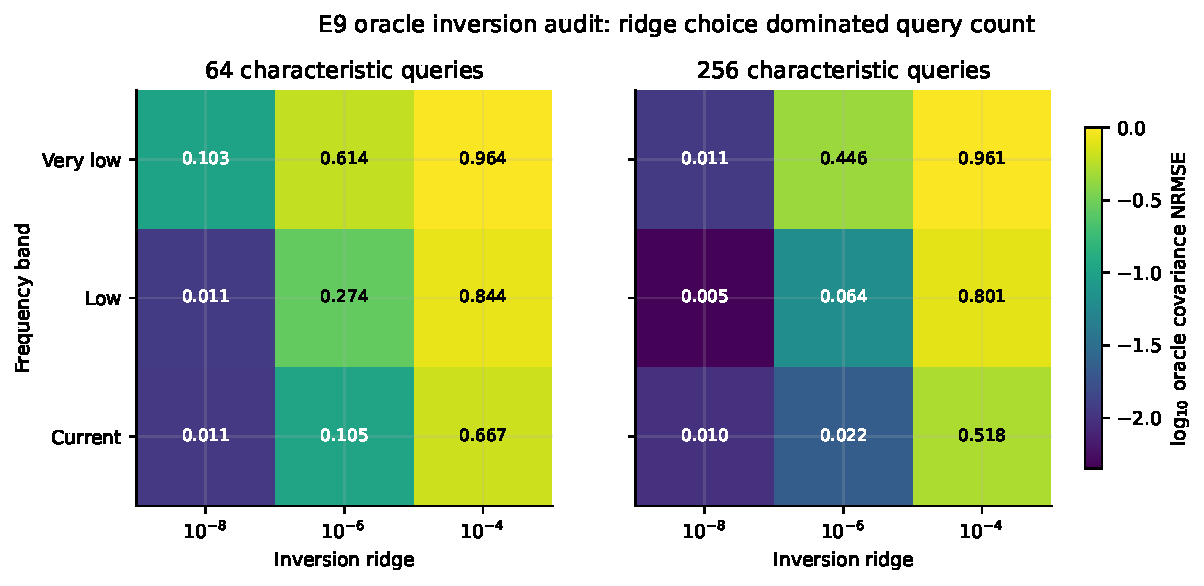
\includegraphics[width=0.96\textwidth]{e9_oracle_inversion_heatmap.pdf}
\caption{E9 oracle readout.  Four orders of magnitude in ridge mattered more than increasing the query count.  Oracle sweeps diagnose readout bias separately from feature-estimation noise.}
\end{figure}

\begin{figure}[t]
\centering
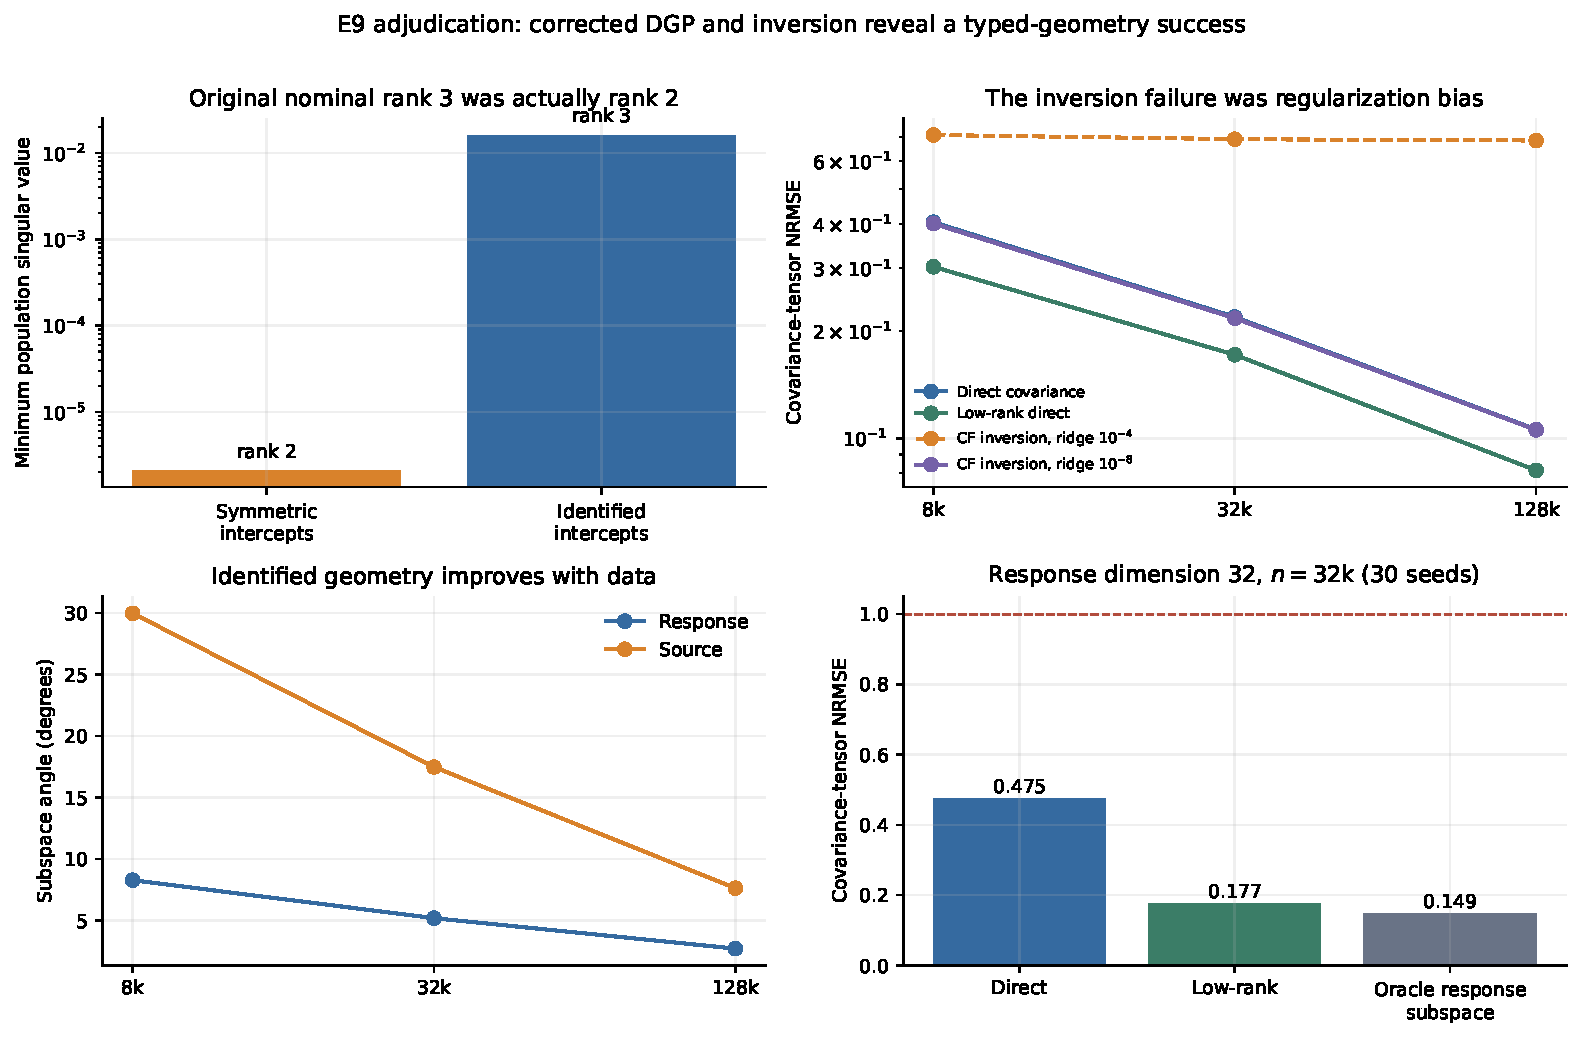
\includegraphics[width=\textwidth]{e9_identification_scaling.pdf}
\caption{E9 diagnosis.  Identified geometry and corrected inverse ridge convert the typed covariance result from apparent failure to sample-scaling success.  Low-rank structure is essential at response dimension 32.}
\end{figure}

\subsection{What succeeds after correction}

In the identified $d_Y=8$ design, ORTH direct covariance NRMSE decreases from 0.404 to 0.219 to 0.106 at $n=8$k, 32k, and 128k.  Response-subspace angles decrease from 8.29 to 5.20 to 2.73 degrees; source angles decrease from 30.0 to 17.5 to 7.64 degrees.  Effective-rank projection further reduces NRMSE to 0.303, 0.172, and 0.081.  The corrected characteristic inverse gives essentially the same typed covariance NRMSE, 0.401, 0.217, and 0.106, showing that inversion can work but gives no point-error advantage over the direct head.

The native characteristic feature tensor remains much harder: ORTH feature NRMSE is 3.97, 1.93, and 1.01 along the same sample ladder.  Increasing from 64 to 256 queries at $n=32$k does not improve the typed covariance result (0.218) and worsens native feature NRMSE to 2.93 because query-estimation noise, not oracle inverse bias, becomes dominant.  The defensible claim is therefore typed covariance geometry, not arbitrary full-law Jacobian recovery.

At $d_Y=32,n=32$k, the 30-seed replication gives ORTH direct NRMSE 0.475 and low-rank NRMSE 0.177; the oracle response-subspace projection is 0.149.  Mean coordinatewise coverage is 0.949.  Null-edge familywise calls occur in 3/30 seeds (0.10; exact 95\% binomial interval 0.021--0.265), so point geometry passes but simultaneous inference is not yet a clean 0.05 result.  PLUG has similar point error but calls the null in every seed because its naive standard error omits nuisance refit uncertainty.  This is a reason to keep ORTH/RIESZ inference even when a direct head supplies the point estimate.

\section{Baseline completeness and the generative-model tangent}

\subsection{Core equal-target baselines}

Every applicable core experiment now contains PLUG, RIESZ-only, and ORTH.  Oracle regression, oracle representer/Riesz, and zero controls appear wherever they isolate a component or normalize NRMSE.  Direct target heads cover mean/moment and covariance subproblems.  E8 contains latent oracle, point projection, exact characteristic correction, and known/estimated measurement variants.  E9 contains direct, effective-low-rank, oracle-subspace, and characteristic-inversion readouts.

\subsection{Flexible reusable-law baselines}

E10 includes full-covariance MDNs with 5/10/20 components and normalized spline flows with 6/10 transforms across all seven required families.  It uses ten DGP seeds, three neural initializations, common evaluation histories, and sampling budgets 64/256/1024.  The analytic MDN readout avoids Monte Carlo derivative noise.  This is 30 neural fits per method/family cell at the frozen local budget; another identical tournament would not adjudicate E6--E9 and was not rerun.

\begin{table}[t]
\centering
\footnotesize
\caption{E10 mean tangent NRMSE from the original complete local tournament.  Bold is the lowest mean, not necessarily a statistically decisive winner.}
\begin{tabular}{@{}lrrrrrr@{}}
\toprule
Family & ORTH & MDN-A5 & MDN-A10 & MDN-A20 & NSF-6 & NSF-10 \\
\midrule
E1 Gaussian & 0.160 & \textbf{0.150} & 0.151 & 0.163 & 0.179 & 0.178 \\
E4 discrete & \textbf{0.235} & 1.082 & 1.063 & 1.057 & 0.431 & 0.413 \\
E4 continuous & \textbf{0.707} & 1.197 & 1.082 & 0.939 & 1.115 & 1.223 \\
E5 support motion & 0.021 & 0.028 & 0.023 & \textbf{0.018} & 0.030 & 0.033 \\
E8 filtered & \textbf{0.688} & 1.050 & 1.097 & 1.074 & 1.126 & 1.216 \\
E9 dense & 6.280 & 6.317 & 4.920 & \textbf{3.890} & 10.015 & 10.160 \\
E11 ordering & \textbf{0.279} & 0.914 & 0.956 & 0.968 & 0.789 & 0.719 \\
\bottomrule
\end{tabular}

\end{table}

\begin{figure}[t]
\centering
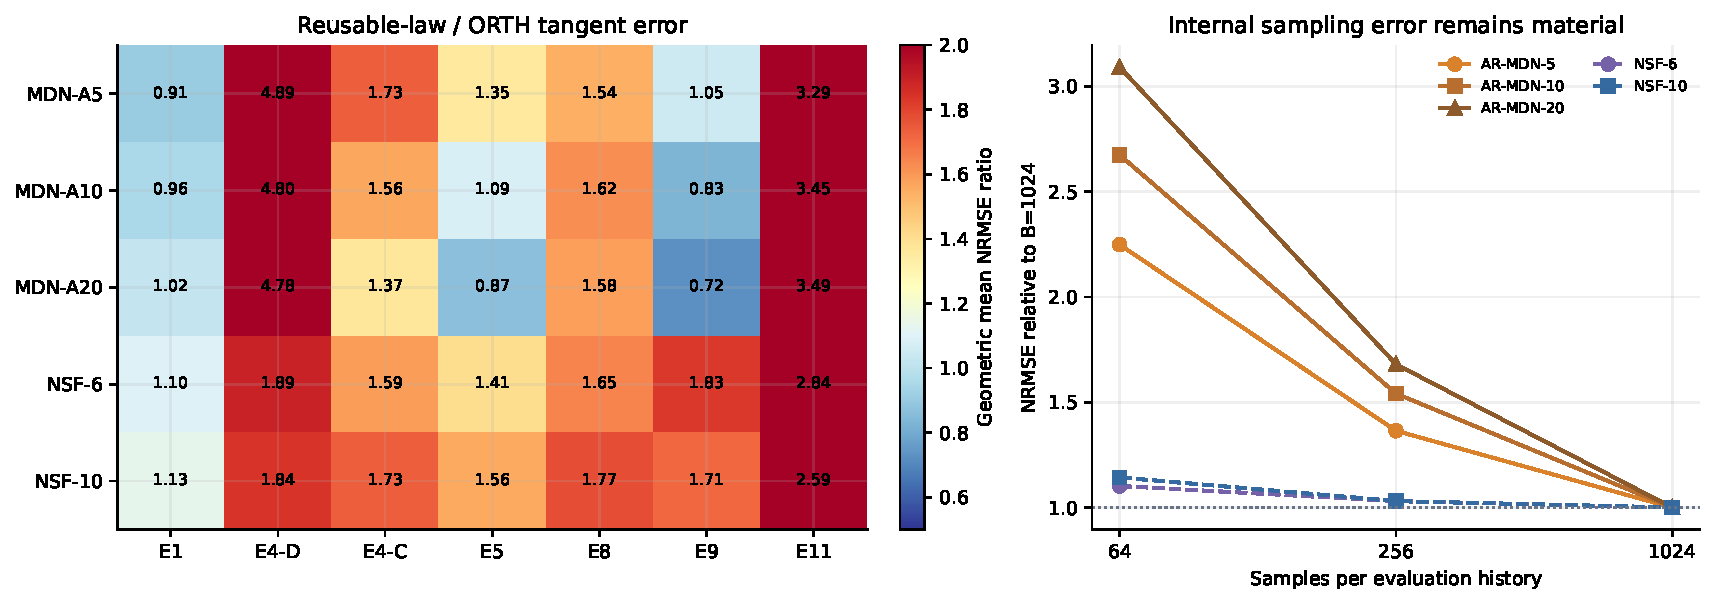
\includegraphics[width=\textwidth]{e10_full_tournament.pdf}
\caption{E10.  ORTH wins the pooled local-budget comparison and the moment-blind/path families.  Analytic MDNs have lower means in some smooth or typed cells; no method is universal.}
\end{figure}

\subsection{Diffusion, denoising-score, flow-matching, and finite contrasts}

These methods were already run in the earlier eight-family history-tangent benchmark: legacy diffusion, EDM diffusion, Gaussian-anchored diffusion, Gaussian DSM, conditional flow matching, affine flow, autoregressive MDN/transformer, Gaussian NLL, bounded energy, and ratio critic.  Stabilization included response standardization, bounded noise ladders, Gaussian anchoring/source choices, gradient clipping, exponential moving averages, and checkpoint selection.  The important result was negative: stable native/generative objectives did not translate into reliable mixed history derivatives.  Across the heterogeneous grid, median tangent NRMSE was 0.616 for the ratio critic, 0.946 for affine flow, 1.015 for the AR MDN, 1.022 for legacy diffusion, 1.260 for Gaussian DSM, 1.743 for EDM diffusion, and 2.692 for anchored diffusion.  These pooled medians are descriptive rather than a paired leaderboard, but they explain why another response-score expansion was not the next decisive experiment.

\begin{figure}[t]
\centering
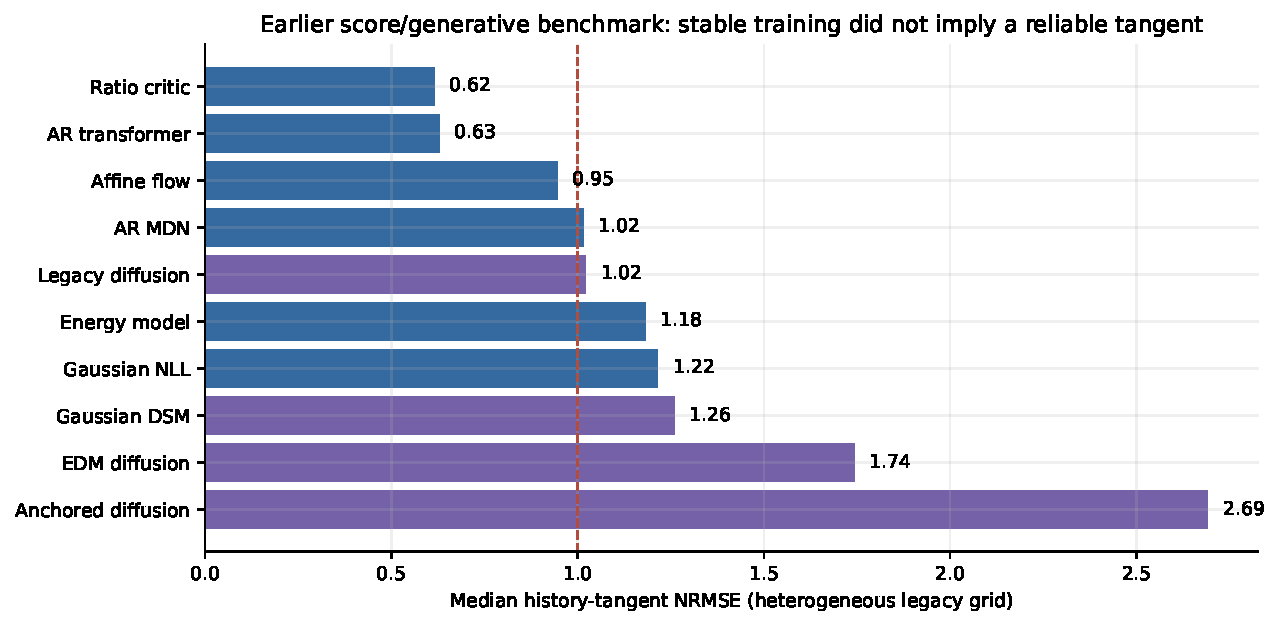
\includegraphics[width=0.86\textwidth]{legacy_score_model_summary.pdf}
\caption{Earlier stabilized score/generative benchmark.  Native training stability and sample quality were insufficient guarantees for the history-tangent target.  The grid and estimand differ from E10, so this is context rather than a new paired comparison.}
\end{figure}

Finite-contrast methods were also run separately: central model log ratios, direct coupled samples, signed classifiers, signed Riesz dictionaries, oracle finite witnesses, and raw history-tangent approximations over multiple $\delta$.  They estimate $P(Y\mid h+\delta v)$ versus $P(Y\mid h-\delta v)$, not $\partial_hP(Y\mid h)$.  They are alternatives when the scientific question is a finite perturbation, not missing same-target baselines for the observational derivative.  The full coverage inventory is in \path{tables/baseline_coverage.csv}.

\clearpage
\section{Consolidated method choice}

\begin{table}[t]
\centering
\footnotesize
\renewcommand{\arraystretch}{1.14}
\caption{Best-supported choice by scientific subproblem.}
\begin{tabularx}{\textwidth}{@{}p{3.0cm}p{2.75cm}p{2.7cm}Y@{}}
\toprule
Problem & Best current method & Why & Main limitation \\
\midrule
Known conditional mean/moment & Direct calibrated head & Lowest variance and simplest target & Not reusable for unanticipated downstream queries \\
Many bounded law queries & Cross-fitted ORTH feature head & Reusable, bounded, calibrated in regular cells & Bank resolution and Riesz quality must be diagnosed \\
Heavy-tail/overlap derivative & Density-score Riesz + ORTH & Removes fixed-sieve bias in E6 sample ladder & Only low-dimensional learned-density evidence so far \\
Moment-blind law change & ORTH characteristic features & Detects changes first four moments miss & Only at frequencies actually queried \\
Deterministic/support motion & ORTH weak features & Remains regular without an ordinary likelihood score & Target is a weak feature derivative, not density score \\
History-local cancellation & ORTH with $R\ge2$ basis & Resolves sign reversals hidden globally & Resolution-variance tradeoff \\
Filtered latent target & Measurement-aware exact CF ORTH & Works when horizon/model make inverse stable & Severe short-horizon and misspecification failures \\
Dense covariance geometry & Direct low-rank covariance + ORTH inference & Best typed error and sample scaling & Requires structural target; null FWER needs more calibration \\
Arbitrary normalized-law reuse & Analytic MDN / NSF & Normalized density and flexible downstream sampling & Tangent quality varies; sampling readout can dominate \\
Finite intervention-like contrast & Ratio/classifier estimator & Targets the actual finite perturbation & Different estimand and no automatic causal interpretation \\
\bottomrule
\end{tabularx}
\end{table}

\section{Theory and empirical synthesis}

\paragraph{The orthogonal-score theory survived.}
E0/E2 validate the algebra and product remainder, E5 validates the weak-feature motivation, and E6 rescue works by improving the nuisance while leaving the score unchanged.  There is no evidence that the basic ORTH functional is the source of the failures.

\paragraph{Orthogonality is robustness, not magic.}
It protects against first-order \emph{shrinking} nuisance errors.  It cannot repair a fixed representer approximation, an unresolved feature bank, an unidentified population rank, or a measurement operator that destroys the queried information.  Each of those failures requires changing a different module.

\paragraph{Representation and readout are part of the estimand.}
E4 shows that frequency coverage determines which law changes exist at the declared resolution.  E9 shows that an invertible population characteristic representation can still be statistically inferior to a typed head after finite-sample noise.  ``Full-law'' should mean a declared finite/multiscale feature family, not unrestricted recovery.

\paragraph{Measurement correction needs a condition number.}
E8 demonstrates that knowing or accurately fitting a filter parameter does not ensure stable latent recovery.  The inverse attenuation and horizon must be reported with every corrected result.  A refusal/partial-identification result is scientifically preferable to a high-variance point estimate.

\paragraph{Generative quality and tangent quality are different axes.}
Diffusion and flow objectives can estimate a conditional law or noisy response score well while the mixed derivative with respect to history remains inaccurate.  A generative model should enter this program only if its tangent is evaluated directly, using analytic/reparameterized derivatives where possible and the same typed/feature metrics as ORTH.

\section{What should be run next}

The broad rerun phase is finished.  The next experiments should be new falsification tests, not more seeds on the same home-field cells.

\begin{enumerate}
\item \textbf{Freeze a high-dimensional E6 confirmation.}  Use nonlinear trajectory histories with $d_H\in\{16,64,256\}$, correlated heavy tails, manifold-plus-noise support, and rare bridges.  Compare targeted neural/RKHS Riesz, diffusion/score-based history-density estimation, sliced/Stein score estimators, and weighted/truncated estimands.  Tune only on probe residuals; confirm on unused DGP families.  Report representer norm, held-out Stein discrepancy, target bias, coverage, and refusal power.
\item \textbf{Misspecify E8 on purpose.}  Generate nonlinear saturation, non-Gaussian shot noise, state-dependent kinetics, unknown cross-talk, and history-dependent missingness while fitting simpler models.  Cross horizon, condition number, and sample size.  Compare exact matched correction, robust/sandwich correction, simulation-based measurement likelihood, partial-identification intervals, and observed-law-only reporting.
\item \textbf{Joint low-rank E9 estimation.}  Fit the response/source subspaces and coefficient functions jointly with nuclear/group penalties rather than projecting a noisy full tensor afterward.  Compare direct covariance, corrected CF inversion, analytic MDN covariance, and oracle subspaces at $d_Y=32/64/128$.  Freeze effective-rank rules and calibrate null FWER on at least 100 null seeds.
\item \textbf{A true sample/compute frontier.}  For ORTH, analytic MDN, NSF, and one stabilized diffusion/flow-matching model, cross $n$, optimization steps, width/depth, evaluation histories, and derivative sampling budget.  Measure likelihood/energy score and tangent error separately.  The question is whether reusable laws close the tangent gap with scale, not which model wins at one arbitrary budget.
\item \textbf{Adaptive multiscale features with honest inference.}  Split selection and inference: use development histories to choose frequencies/witnesses, then freeze the bank for held-out estimation.  Compare fixed random Fourier, learned witness, wavelet/path, and typed hybrid banks.  Report stability across banks, not only the best selected result.
\end{enumerate}

\section{Limitations and claim boundary}

The E6 density-score rescue is low-dimensional and uses a flexible mixture density; it may fail in realistic trajectory spaces.  E8's strongest rescue is correctly specified and therefore a best-case identifiability demonstration, not robustness evidence.  E9's intercept change is a post-hoc correction to the synthetic design; its success must be reconfirmed prospectively.  Ten seeds are enough to diagnose large mean-error trends but not to certify 5\% familywise error; even the 30-seed $d_Y=32$ replication leaves a wide interval around its 0.10 call rate.  E10 is a local compute comparison, not a scaling law.  Earlier generative-model medians aggregate heterogeneous strata and are not directly comparable to the new ORTH cells.  None of these synthetic results supports causal, latent biological, or real-neural interpretation without a separate observation and identification argument.

\section{Reproducibility map}

\scriptsize
\begin{longtable}{@{}p{4.0cm}p{3.0cm}p{7.9cm}@{}}
\toprule
Artifact & Purpose & Location relative to repository root \\
\midrule
\endfirsthead
\toprule
Artifact & Purpose & Location relative to repository root \\
\midrule
\endhead
Original decisive report & E0--E11 full confirmation & \path{reports/distributional_sid_decisive_2026-07-14/main.pdf} \\
Adjudication implementation & New E6/E8/E9 experiments & \path{distributional_sid/src/distributional_sid/adjudication_experiments.py} \\
Adjudication tests & Unit/integration checks & \path{distributional_sid/tests/test_adjudication_experiments.py} \\
E6 tuning & Width/ridge development & \path{distributional_sid/runs/e6_adjudication_tuning_20260714} \\
E6 post-hoc & Tail/gap sample scaling & \path{distributional_sid/runs/e6_adjudication_posthoc_20260714} \\
E8 post-hoc & Horizon/data/deconvolution grid & \path{distributional_sid/runs/e8_adjudication_posthoc_20260714} \\
E8 likelihood supplement & Correctly fitted measurement model & \path{distributional_sid/runs/e8_mixture_mle_posthoc_20260714} \\
E9 identifiability & Symmetric versus identified rank & \path{distributional_sid/runs/e9_identifiability_posthoc_20260714} \\
E9 oracle tuning & Query/band/ridge sweep & \path{distributional_sid/runs/e9_oracle_inversion_tuning_20260714} \\
E9 corrected inverse & Ridge-$10^{-8}$ sample scaling & \path{distributional_sid/runs/e9_inversion_ridge_posthoc_20260714} \\
E9 query stress & 256-query check & \path{distributional_sid/runs/e9_query256_posthoc_20260714} \\
E9 high dimension & $d_Y=32$, 30-seed pooled replication & \path{distributional_sid/runs/e9_response32_direct_*_20260714} \\
E10 flexible laws & MDN/NSF complete tournament & \path{distributional_sid/runs/e10_full_confirmation_20260714} and \path{e10_analytic_mdn_confirmation_20260714} \\
Earlier generative grid & Diffusion/DSM/flow/ratio tangent results & \path{history_tangent_benchmark/results/stable_sid_core_20260713} \\
Earlier finite grid & Ratio/classifier/Riesz finite contrasts & \path{history_tangent_benchmark/results/stable_sid_finite_20260713} \\
Machine-readable summaries & Gate, baseline, validation, E6--E9 tables & \path{reports/distributional_sid_adjudication_2026-07-14/tables} \\
Snapshot & Key values and decisions & \path{reports/distributional_sid_adjudication_2026-07-14/results_snapshot.json} \\
\bottomrule
\end{longtable}
\normalsize

\section{Final decision}

There is a coherent, promising method here, but it is not a single universal estimator.  The core contribution should be framed as a modular theory of \emph{declared predictive-feature derivatives}: bounded feature regression provides the future-law representation, history-side Riesz/score learning identifies average derivatives, and cross-fitted orthogonalization provides robust inference.  Structured typed heads, measurement operators, and finite contrasts are complementary modules chosen by the scientific target.

The best current empirical claim is: under diagnosed history support, a resolving bounded feature representation, and a sufficiently informative observation process, ORTH estimates predictive distributional derivatives with useful calibration and distinctive advantages for support motion, moment-blind changes, heterogeneity, and path order.  The strongest repaired extensions are density-score Riesz learning in low-dimensional tail/overlap stress and direct low-rank covariance geometry.  The claims that remain unsupported are unrestricted high-dimensional history-score estimation, robustness to measurement misspecification, arbitrary full-law Jacobian recovery, and latent/causal neural interpretation.

\end{document}
